\section{Dynamic Response Analysis Using Newmark-{$\beta$} Method}

\subsection{Problem Definition}

A linear single-degree-of-freedom (SDOF) system is defined by:

\begin{align}
m &= 3600 \ \text{kg} \\
k &= 1400 \ \text{kN/m} = 1.4 \times 10^6 \ \text{N/m} \\
c &= 70 \ \text{kN·s/m} = 7.0 \times 10^4 \ \text{N·s/m}
\end{align}

The system is subjected to a time-varying external force $F(t)$ as shown in the assignment. 
The equation of motion is:

\begin{equation}
m\ddot{u}(t) + c\dot{u}(t) + ku(t) = F(t)
\end{equation}

The system is initially at rest:

\begin{equation}
u(0) = 0, \quad \dot{u}(0) = 0
\end{equation}

---

\subsection{Newmark-$\beta$ Method}

The Newmark-$\beta$ method with constant average acceleration is used:

\begin{equation}
\beta = \frac{1}{4}, \quad \gamma = \frac{1}{2}
\end{equation}

For the constant average acceleration method ($\beta = 1/4$, $\gamma = 1/2$), the following constants are defined:

\begin{align}
a_0 &= \frac{1}{\beta \Delta t^2}, &
a_1 &= \frac{\gamma}{\beta \Delta t}, \\
a_2 &= \frac{1}{\beta \Delta t}, &
a_3 &= \frac{1}{2\beta} - 1, \\
a_4 &= \frac{\gamma}{\beta} - 1, &
a_5 &= \Delta t \left(\frac{\gamma}{2\beta} - 1\right)
\end{align}

For $\Delta t = 0.1$ s:

\begin{equation}
a_0 = 400, \quad a_1 = 20, \quad a_2 = 40, \quad a_3 = 1, \quad a_4 = 1, \quad a_5 = 0
\end{equation}

The method leads to the following recurrence relations:

\begin{align}
u_{i+1} &= \frac{\hat{F}_{i+1}}{k_{\text{eff}}} \\
\ddot{u}_{i+1} &= a_0(u_{i+1} - u_i) - a_2 \dot{u}_i - a_3 \ddot{u}_i \\
\dot{u}_{i+1} &= \dot{u}_i + \Delta t \left[(1-\gamma)\ddot{u}_i + \gamma \ddot{u}_{i+1} \right]
\end{align}

where the effective force is:

\begin{equation}
\hat{F}_{i+1} =
F_{i+1}
+ m(a_0 u_i + a_2 \dot{u}_i + a_3 \ddot{u}_i)
+ c(a_1 u_i + a_4 \dot{u}_i + a_5 \ddot{u}_i)
\end{equation}

and the effective stiffness is:

\begin{equation}
k_{\text{eff}} = k + a_0 m + a_1 c
\end{equation}

For $\Delta t = 0.1$ s,

\begin{equation}
k_{\text{eff}} = 1.4 \times 10^6 + 400(3600) + 20(70000) = 4.24 \times 10^6 \ \text{N/m}
\end{equation}

---

\subsection{Time Integration Parameters}

\begin{equation}
\Delta t = 0.1 \ \text{s}, \quad t_{\text{end}} = 2.0 \ \text{s}
\end{equation}

The loading is applied for $t \leq 1.0$ s and set to zero afterward, resulting in free vibration beyond this point.

---

\subsection{Numerical Implementation}

The response was computed using a Python implementation of the Newmark-$\beta$ method. 
The algorithm evaluates displacement, velocity, and acceleration at each time step. 
An Excel file was also used to verify and validate the results.

---

\subsection{Results}

The response was computed for two time steps, $\Delta t = 0.1$ s and $\Delta t = 0.01$ s.
Requested tabulated outputs are provided below for time, force, displacement, velocity, acceleration, and effective force.

As a consistency check, the maximum static displacement is estimated as:

\begin{equation}
u_{\text{static}} = \frac{F_{\max}}{k}
= \frac{40000}{1.4 \times 10^6}
\approx 2.86 \times 10^{-2} \ \text{m}
\end{equation}

The computed maximum dynamic displacement is approximately:

\begin{equation}
u_{\max} \approx 3.06 \times 10^{-2} \ \text{m}
\end{equation}

The dynamic displacement is slightly larger than the static estimate, which is expected due to dynamic amplification effects.

The natural frequency of the system is:

\begin{equation}
\omega_n = \sqrt{\frac{k}{m}} = \sqrt{\frac{1.4 \times 10^6}{3600}} \approx 19.7 \ \text{rad/s}
\end{equation}

The corresponding natural period is:

\begin{equation}
T_n = \frac{2\pi}{\omega_n} \approx 0.319 \ \text{s}
\end{equation}

The oscillation period observed in the response plots is consistent with this value.

\subsubsection{Table for $\Delta t = 0.1$ s}

\begin{table}[H]
\centering
\scriptsize
\caption{Response history for $\Delta t = 0.1$ s}
\begin{tabular}{rrrrrr}
\hline
$t$ (s) & $F$ (N) & $u$ (m) & $\dot{u}$ (m/s) & $\ddot{u}$ (m/s$^2$) & $\hat{F}$ (N) \\
\hline
0.00 & 0 & 0.000000e+00 & 0.000000e+00 & 0.000000e+00 & 0.00 \\
0.10 & 8000 & 1.886792e-03 & 3.773585e-02 & 7.547170e-01 & 8000.00 \\
0.20 & 18000 & 8.054468e-03 & 8.561766e-02 & 2.029192e-01 & 34150.94 \\
0.30 & 36000 & 1.837910e-02 & 1.208750e-01 & 5.022267e-01 & 77927.38 \\
0.40 & 39000 & 2.803582e-02 & 7.225957e-02 & -1.474534e+00 & 118871.89 \\
0.50 & 40000 & 3.060777e-02 & -2.082056e-02 & -3.870682e-01 & 129776.96 \\
0.60 & 39000 & 2.832006e-02 & -2.493383e-02 & 3.048028e-01 & 120077.04 \\
0.70 & 31000 & 2.528076e-02 & -3.585215e-02 & -5.231692e-01 & 107190.41 \\
0.80 & 19000 & 1.916075e-02 & -8.654799e-02 & -4.907475e-01 & 81241.58 \\
0.90 & 10000 & 1.040768e-02 & -8.851338e-02 & 4.514396e-01 & 44128.57 \\
1.00 & 0 & 2.887060e-03 & -6.189905e-02 & 8.084708e-02 & 12241.13 \\
1.10 & 0 & -1.121721e-03 & -1.827657e-02 & 7.916025e-01 & -4756.10 \\
1.20 & 0 & -1.001675e-03 & 2.067748e-02 & -1.252160e-02 & -4247.10 \\
1.30 & 0 & 3.620623e-04 & 6.597278e-03 & -2.690824e-01 & 1535.14 \\
1.40 & 0 & 3.470230e-04 & -6.898063e-03 & -8.244064e-04 & 1471.38 \\
1.50 & 0 & -1.164169e-04 & -2.370737e-03 & 9.137092e-02 & -493.61 \\
1.60 & 0 & -1.200534e-04 & 2.298007e-03 & 2.003967e-03 & -509.03 \\
1.70 & 0 & 3.727267e-05 & 8.485146e-04 & -3.099382e-02 & 158.04 \\
1.80 & 0 & 4.147612e-05 & -7.644456e-04 & -1.265382e-03 & 175.86 \\
1.90 & 0 & -1.187608e-05 & -3.025983e-04 & 1.050233e-02 & -50.35 \\
2.00 & 0 & -1.431031e-05 & 2.539136e-04 & 6.279094e-04 & -60.68 \\
\hline
\end{tabular}
\end{table}
\FloatBarrier

\subsubsection{Standalone Plots for $\Delta t = 0.1$ s}

\begin{figure}[H]
\centering
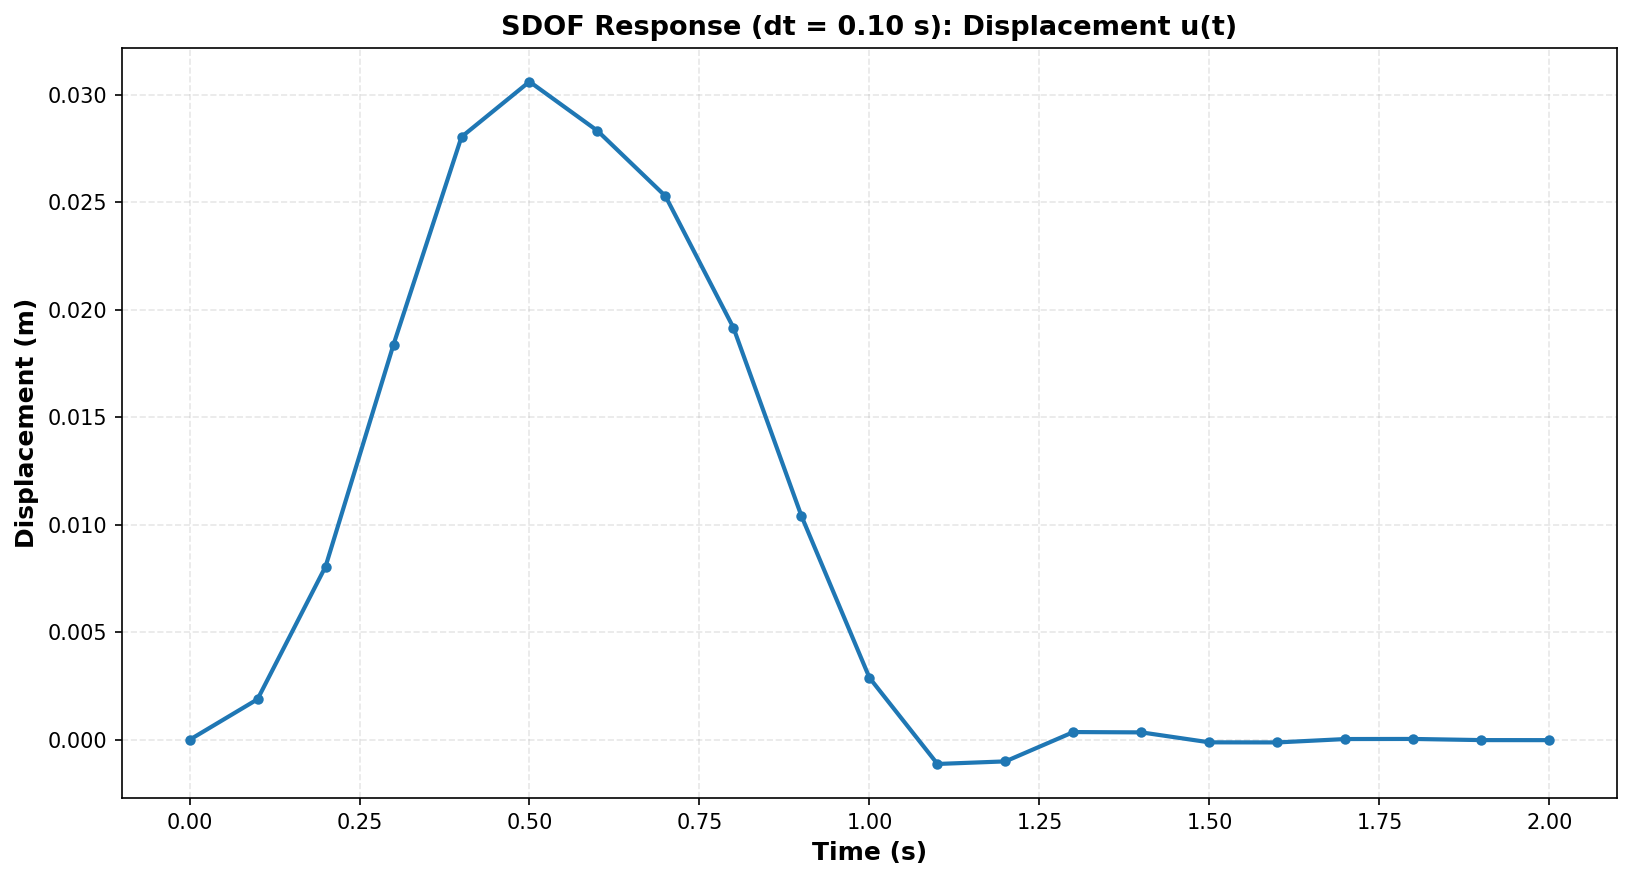
\includegraphics[width=0.8\textwidth]{figures/dt01_displacement.png}
\caption{Displacement response for $\Delta t = 0.1$ s}
\end{figure}

\begin{figure}[H]
\centering
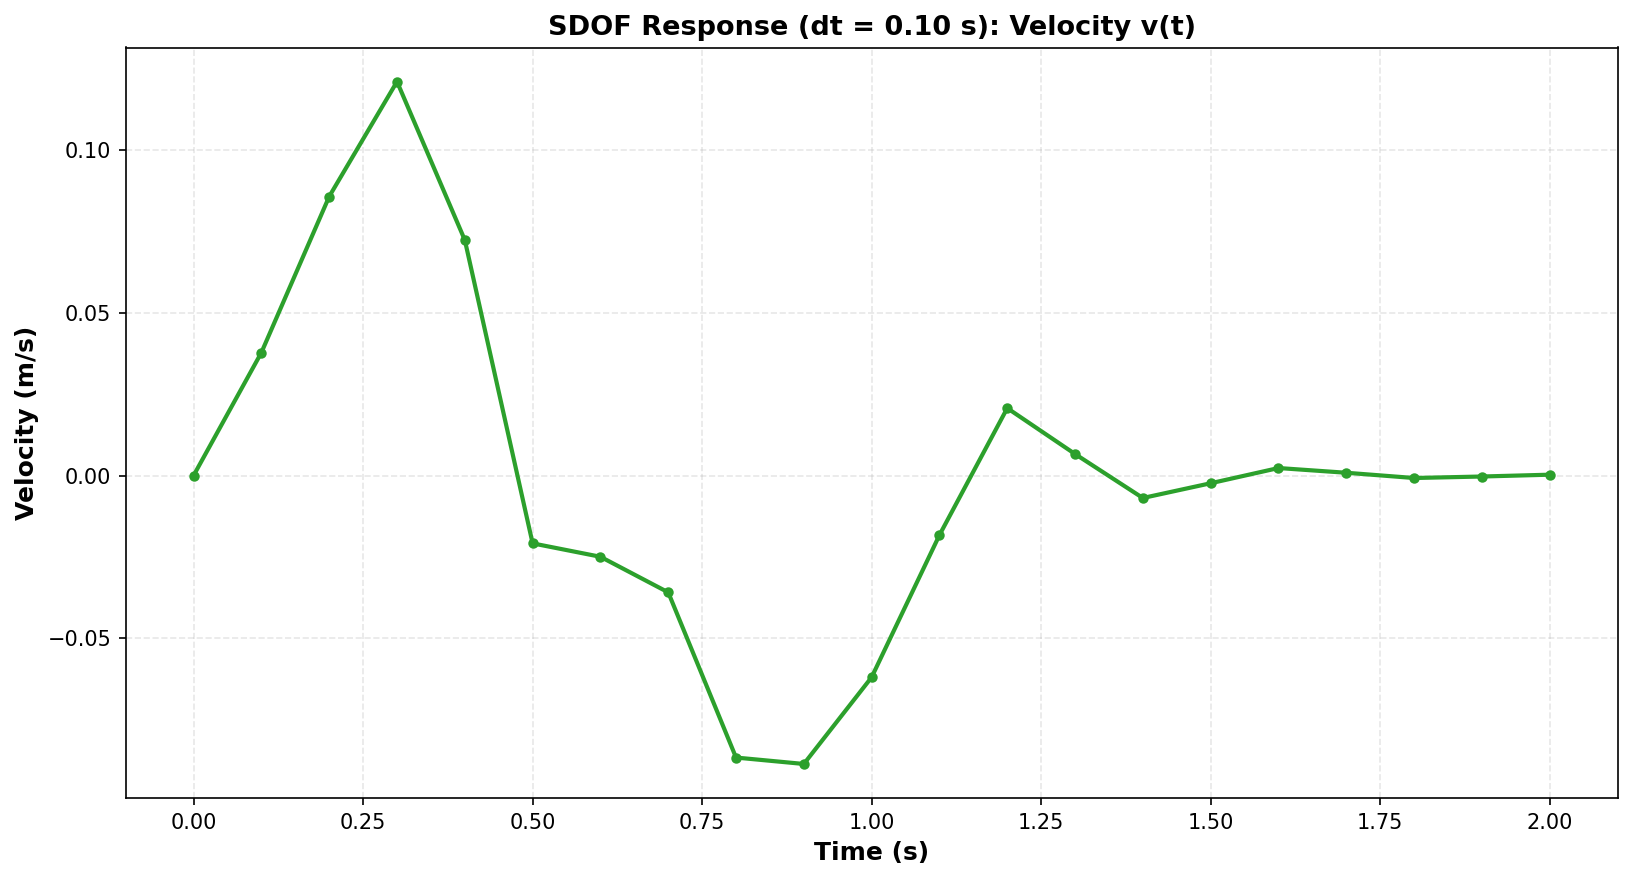
\includegraphics[width=0.8\textwidth]{figures/dt01_velocity.png}
\caption{Velocity response for $\Delta t = 0.1$ s}
\end{figure}

\begin{figure}[H]
\centering
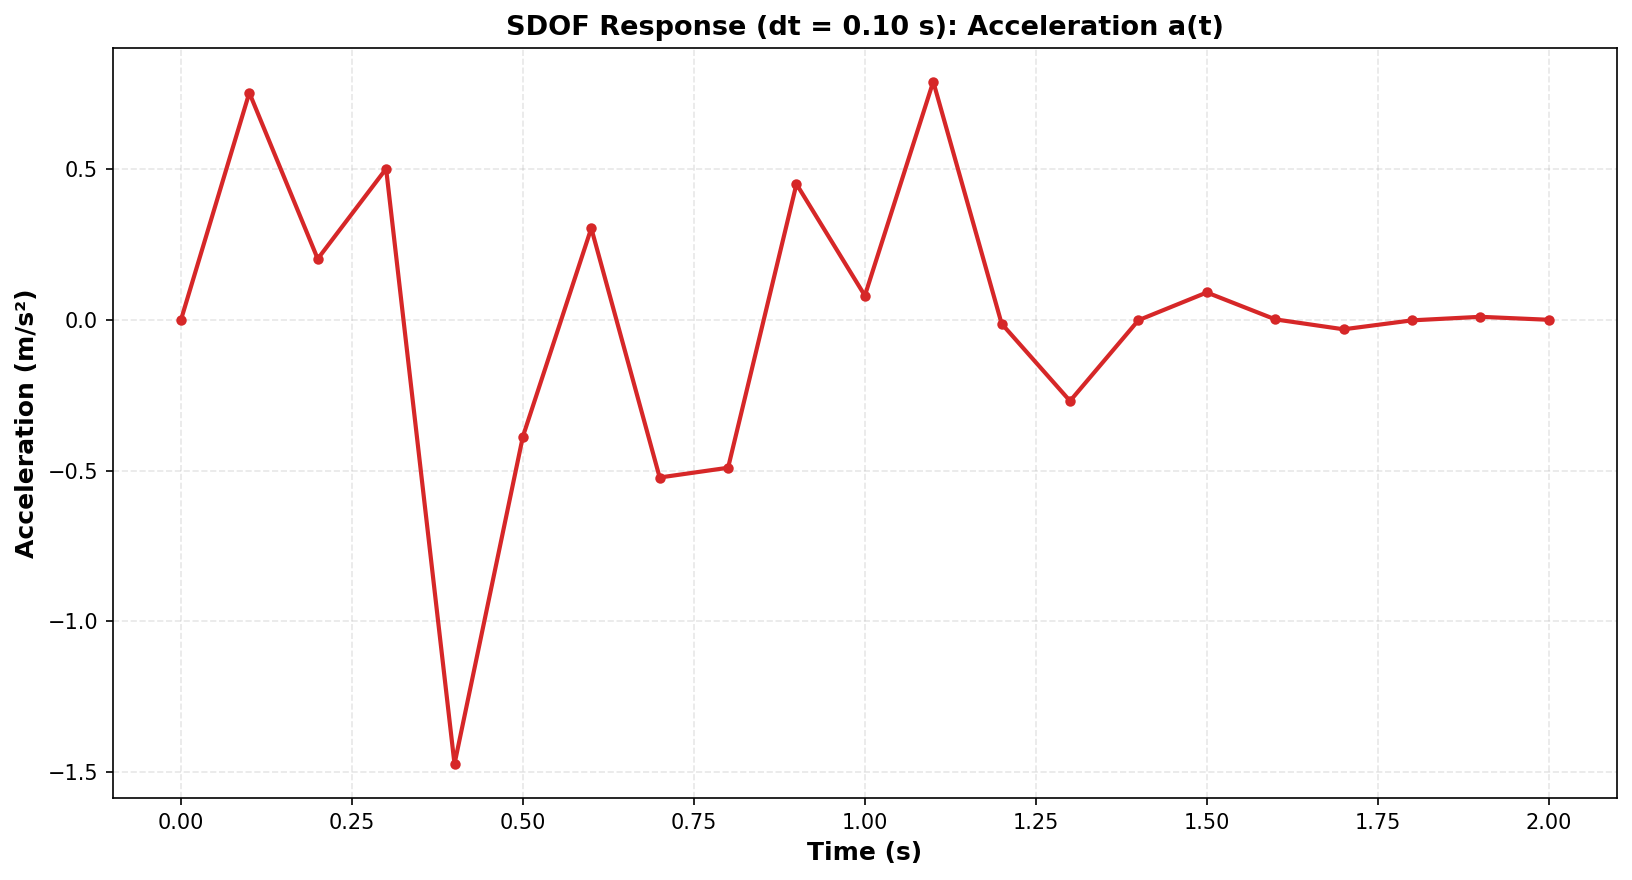
\includegraphics[width=0.8\textwidth]{figures/dt01_acceleration.png}
\caption{Acceleration response for $\Delta t = 0.1$ s}
\end{figure}
\FloatBarrier

\subsubsection{Table for $\Delta t = 0.01$ s}

\begin{table}[H]
\centering
\scriptsize
\caption{Sampled response history for $\Delta t = 0.01$ s}
\begin{tabular}{rrrrrr}
\hline
$t$ (s) & $F$ (N) & $u$ (m) & $\dot{u}$ (m/s) & $\ddot{u}$ (m/s$^2$) & $\hat{F}$ (N) \\
\hline
0.00 & 0 & 0.000000e+00 & 0.000000e+00 & 0.000000e+00 & 0.00 \\
0.06 & 4800 & 5.747266e-04 & 2.510103e-02 & 6.217529e-01 & 91611.42 \\
0.12 & 10000 & 3.112619e-03 & 5.752280e-02 & 4.488160e-01 & 496151.42 \\
0.18 & 16000 & 7.210806e-03 & 7.618853e-02 & 1.587986e-01 & 1149402.42 \\
0.24 & 25200 & 1.210734e-02 & 9.170017e-02 & 5.085324e-01 & 1929909.45 \\
0.30 & 36000 & 1.855460e-02 & 1.221247e-01 & 4.096757e-01 & 2957603.00 \\
0.36 & 37800 & 2.533206e-02 & 8.935438e-02 & -1.088801e+00 & 4037929.66 \\
0.42 & 39200 & 2.877302e-02 & 2.810243e-02 & -8.470568e-01 & 4586420.11 \\
0.48 & 39800 & 2.929157e-02 & -4.804142e-03 & -2.421986e-01 & 4669077.05 \\
0.54 & 39600 & 2.880148e-02 & -9.622536e-03 & -1.347094e-02 & 4590956.01 \\
0.60 & 39000 & 2.823385e-02 & -8.910194e-03 & 2.675564e-02 & 4500476.06 \\
0.66 & 34200 & 2.724435e-02 & -2.934867e-02 & -5.243572e-01 & 4342749.72 \\
0.72 & 28600 & 2.459707e-02 & -5.813043e-02 & -4.907698e-01 & 3920773.35 \\
0.78 & 21400 & 2.027747e-02 & -8.397833e-02 & -3.083259e-01 & 3232228.51 \\
0.84 & 15400 & 1.494569e-02 & -8.843267e-02 & 1.850903e-01 & 2382342.50 \\
0.90 & 10000 & 1.009166e-02 & -7.264706e-02 & 2.658258e-01 & 1608610.31 \\
1.00 & 0 & 3.357203e-03 & -6.282655e-02 & 2.129504e-01 & 535194.31 \\
1.20 & 0 & -4.007250e-04 & 1.082452e-02 & -5.463922e-02 & -63875.57 \\
1.40 & 0 & 2.852457e-05 & -1.320617e-03 & 1.698307e-02 & 4548.22 \\
1.60 & 0 & 7.775912e-06 & 2.613269e-04 & -3.373681e-03 & 1239.21 \\
1.80 & 0 & -1.501355e-07 & -2.812460e-05 & 6.052533e-04 & -23.93 \\
2.00 & 0 & 9.216740e-08 & 3.105826e-06 & -9.623394e-05 & 14.69 \\
\hline
\end{tabular}
\end{table}
\FloatBarrier

\subsubsection{Comparison Plots: $\Delta t = 0.01$ s vs $\Delta t = 0.1$ s}

\begin{figure}[H]
\centering
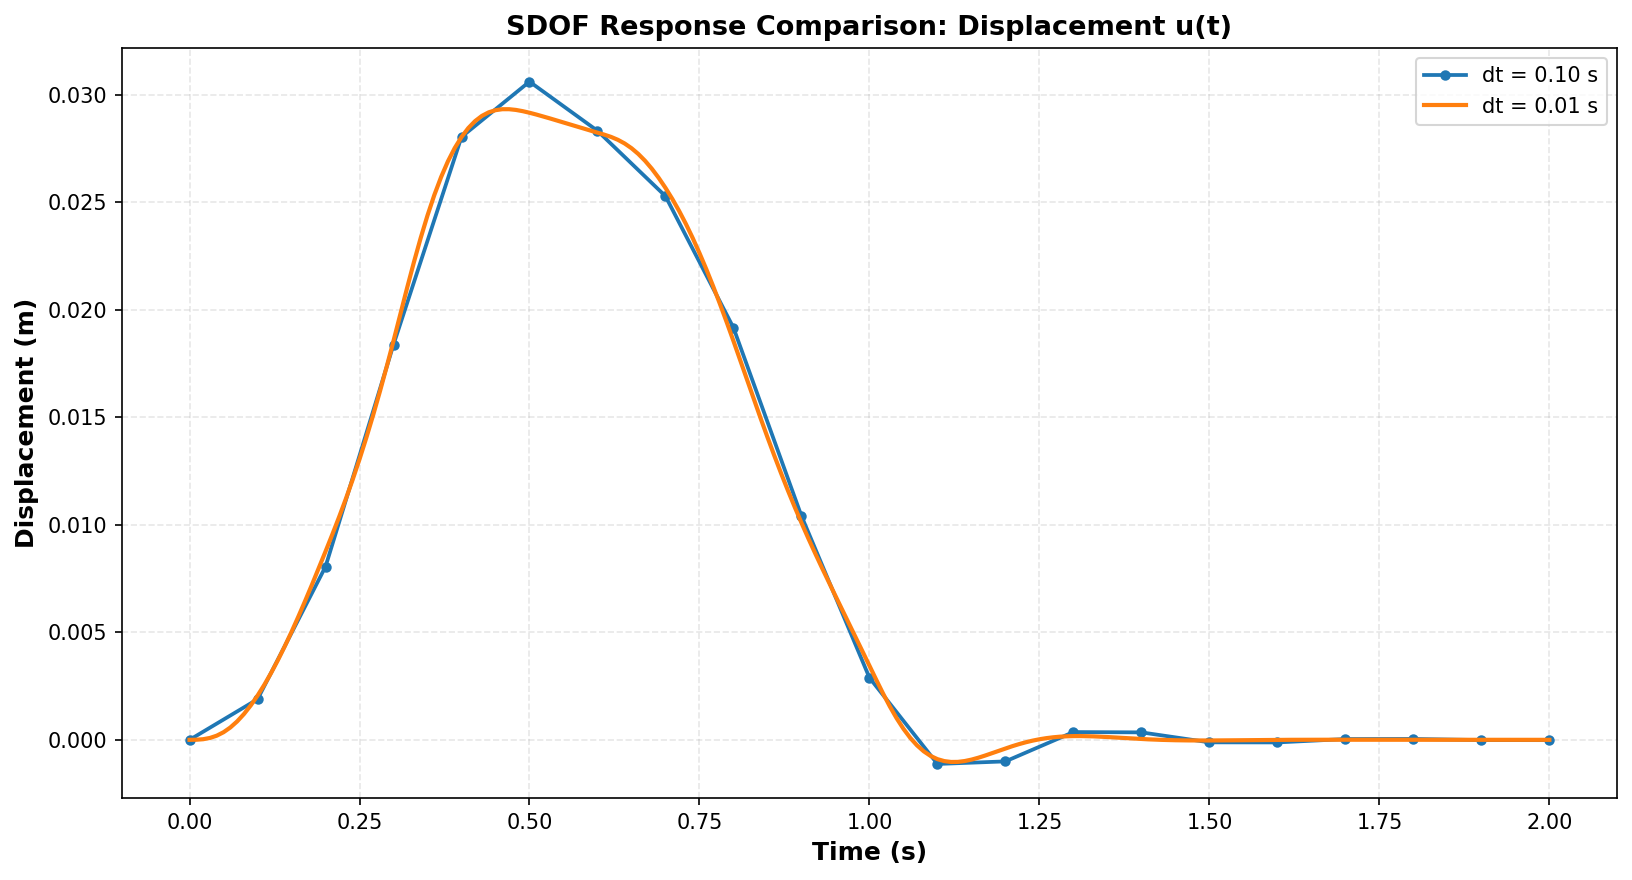
\includegraphics[width=0.8\textwidth]{figures/comparison_displacement.png}
\caption{Displacement comparison between $\Delta t = 0.01$ s and $\Delta t = 0.1$ s}
\end{figure}

\begin{figure}[H]
\centering
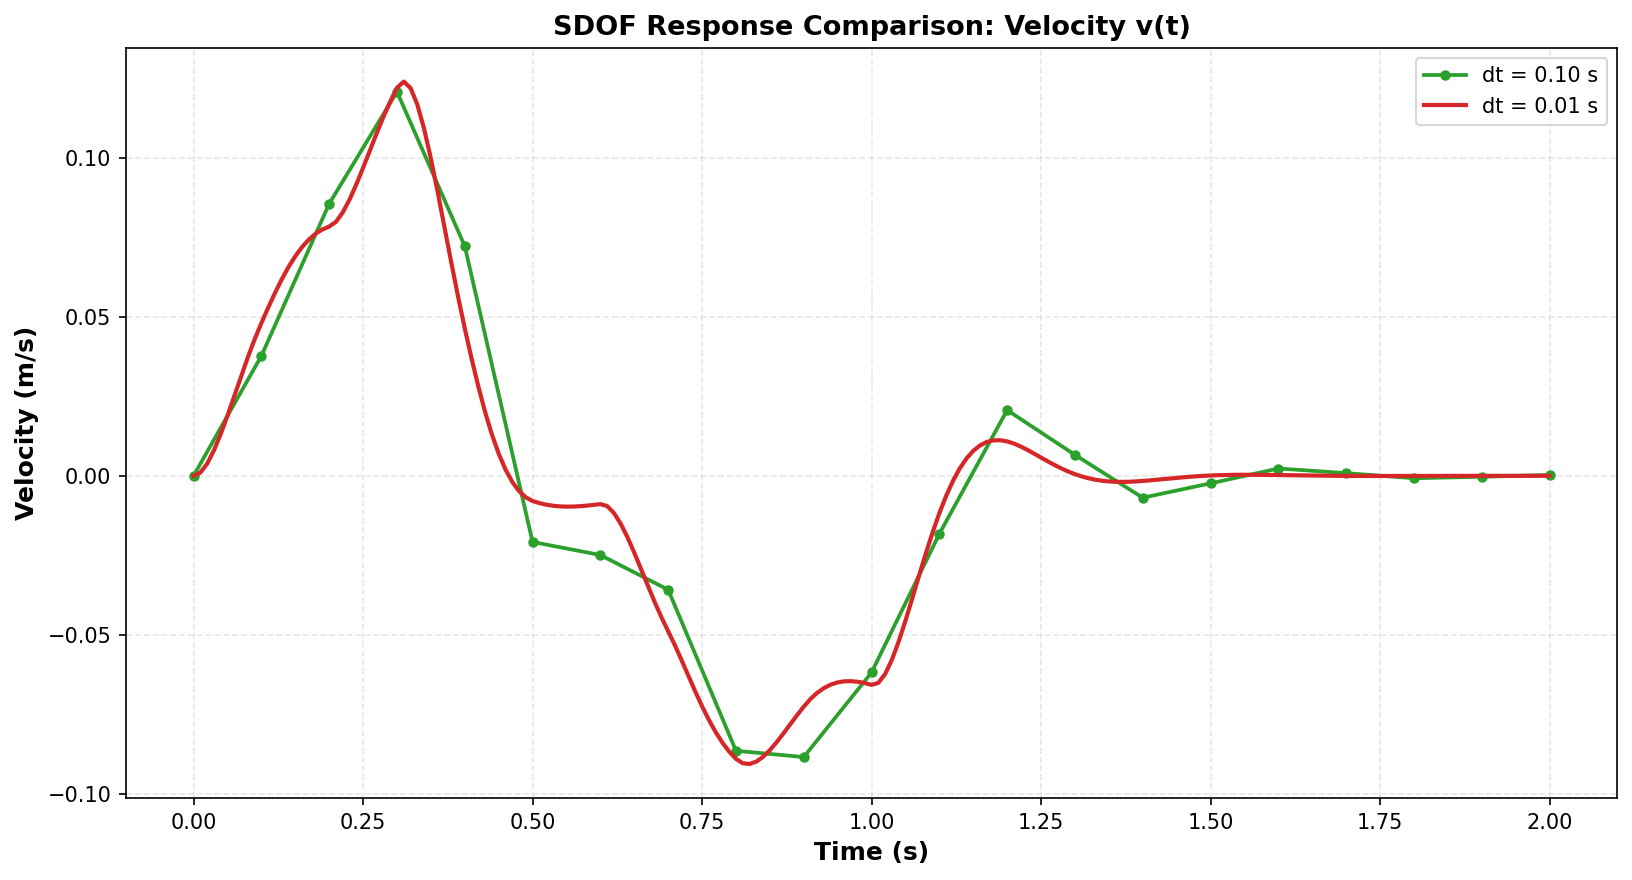
\includegraphics[width=0.8\textwidth]{figures/comparison_velocity.png}
\caption{Velocity comparison between $\Delta t = 0.01$ s and $\Delta t = 0.1$ s}
\end{figure}

\begin{figure}[H]
\centering
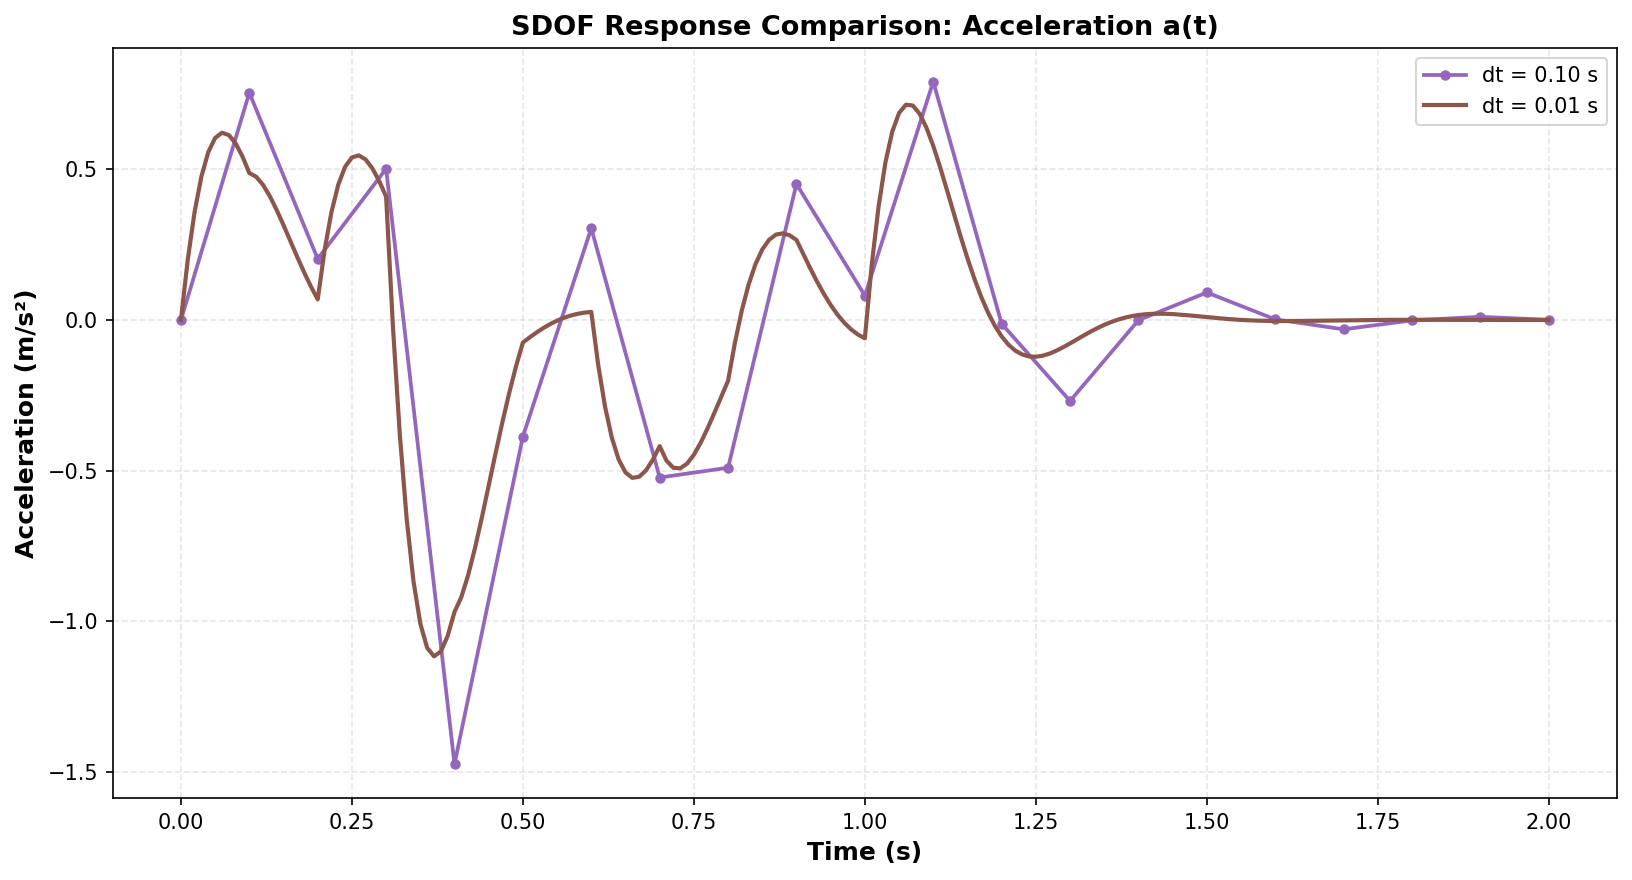
\includegraphics[width=0.8\textwidth]{figures/comparison_acceleration.png}
\caption{Acceleration comparison between $\Delta t = 0.01$ s and $\Delta t = 0.1$ s}
\end{figure}
\FloatBarrier

---

\subsection{Discussion}

The response of the system consists of two distinct phases: forced vibration
for $0 \leq t \leq 1.0$ s and free vibration for $t > 1.0$ s, after the external
loading is removed.

During the forced vibration phase, the displacement increases as the applied
force rises, reaching a peak value of approximately $3.06 \times 10^{-2}$ m at
$t \approx 0.5$ s. This value is slightly higher than the corresponding static
displacement estimate,
\[
u_{\text{static}} = \frac{F_{\max}}{k} \approx 2.86 \times 10^{-2}\ \text{m},
\]
indicating the presence of dynamic amplification due to inertia effects.

The response exhibits oscillatory behavior consistent with the natural period
of the system, $T_n \approx 0.319$ s. The displacement, velocity, and acceleration
plots all reflect this periodic behavior, confirming that the numerical solution
captures the fundamental dynamic characteristics of the system.

After $t = 1.0$ s, the system undergoes free vibration. Due to the presence of
damping ($c = 7.0 \times 10^4$ N·s/m), the amplitude of oscillation gradually
decays over time. By $t = 2.0$ s, the response has nearly diminished, with the
displacement approaching zero and only small residual oscillations remaining.

The comparison between $\Delta t = 0.1$ s and $\Delta t = 0.01$ s shows that both
time steps produce consistent peak values and overall trends. However, the
smaller time step yields a smoother and more refined response, particularly in
the velocity and acceleration histories. This indicates improved numerical
resolution of the dynamic response.

Overall, the results demonstrate that the Newmark-$\beta$ method with constant
average acceleration provides stable and accurate solutions for the given
time-step sizes. The close agreement between the two time steps suggests that
$\Delta t = 0.1$ s is sufficient for capturing the essential behavior of the
system, while $\Delta t = 0.01$ s offers higher fidelity at increased
computational cost.